\documentclass[thesis.tex]{subfiles}
\begin{document}
\chapter{Background}

\begin{todo}
  \begin{itemize}
  \item Describe Android in depth.
  \item Describe App stores and the scale of their use.  Introduce
    the idea that they're somewhat difficult to search and find appropriate
    ones.
  \item \emph{Thorough} review of authorization logics, and static analysis
    results for Android.
  \end{itemize}
\end{todo}

\section{Android and Mobile OSs}\label{android}

Android is a mobile operating system developed, primarily, by Google. It
is by far the most popular mobile operating system in use being
installed on around 83\% of all mobile handsets\footnote{\url{http://www.idc.com/prodserv/smartphone-os-market-share.jsp}}
with Apple's iOS being its only major competitor (Windows Phone,
Blackberry OS and other mobile operating systems account for only 3\% of
the marketshare in 2015).

Despite the dominance of Android its ecosystem is rather fragmented. As
shown in Figure \url{fig:android-versions}, in June 2016 only 10\% of
devices used the latest version of Android, with around 5\% of devices
still using a version released five years prior. The range of different
Android versions is often blamed on the device manufacturers being
unwilling to update their devices. Since the core of Android is open
source this has lead to third parties (such as CyanogenMod\footnote{\url{http://www.cyanogenmod.org}})
have started developing custom firmware for Android devices to allow
older devices to be upgraded independently of their manufacturers.

\begin{figure*}[htbp]
\centering
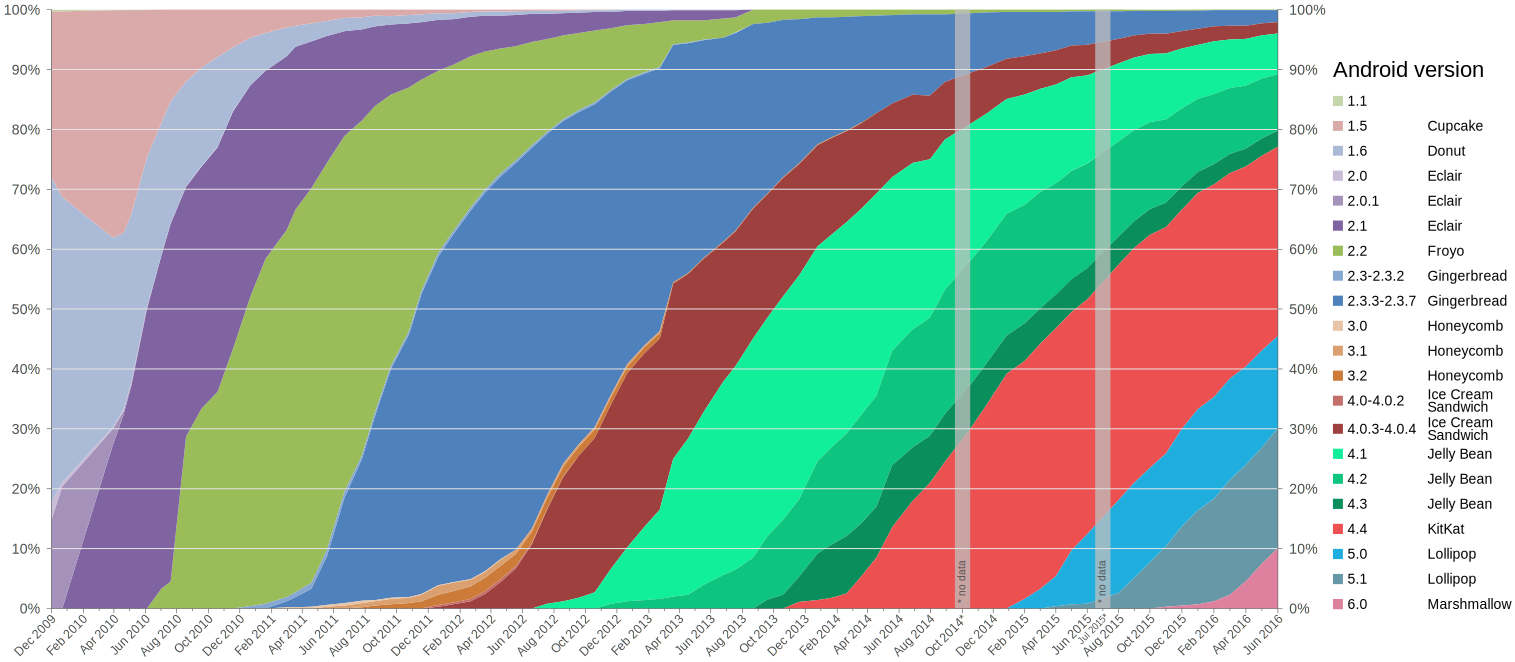
\includegraphics[width=\linewidth]{chapters/02-background/figures/android-versions.eps}
\caption[ Historical Android version's distribution. ]{Historical Android version's distribution. Figure by \emph{Erikrespo} taken from \url{https://en.wikipedia.org/wiki/Android_version_history}.}
\end{figure*}

When building an Android device the manufacturers are also able to make
modifications to the Android firmware. This can be done to support any
custom hardware their device may have, add any additional software or
apps, or provide a custom look or theme to their device. Again this
creates more variety in the ecosystem, with few guarantees that any two
devices may contain similar features or hardware. In fact since the core
of the Android is the Linux kernel (albeit without the Linux Standard
Base\footnote{The \emph{Linux Standard Base} is a specification produced
  by the Linux foundation that describes what a stardard Linux system
  should contain and how it should be organised. Android uses its own
  system which differs most noticably by the different filesystem
  structures and the use of user IDs to separate apps rather than users.
  \url{http://refspecs.linuxfoundation.org/lsb.shtml}}, and with
additional patches) it can be ported to other architectures (such as X86
and MIPS), and used in other devices (such as set-top boxes and TVs,
watches, and cars) with relative ease.

To give developers a somewhat stable base to develop for Google
developed the \emph{Compatibility Test Suite} (CTS)\footnote{\url{https://source.android.com/compatibility/cts/index.html}},
and \emph{Compatibility Definition Document} (CDD)\footnote{\url{https://source.android.com/compatibility/android-cdd.html}}.
The CTS is a series of unit tests that check basic Android functionality
and behavior. The CDD is a document that describes what hardware an
Android device should have and how the device and it's software should
be built. If a device manufacturer wishes their device to run Google's
Play Store (the largest Android app marketplace), then they are required
to show they can pass the CTS and are in compliance with the CDD.

\section{App Stores}\label{app-stores}

The Play Store is Google's marketplace for apps. It contains a large
number of apps (around 2.2 million) uploaded by developers for users to
buy. To use the market places user's can login with a Google account
which is then used to sync purchases to their devices. Developers pay a
small fee (currently \$25) to submit an app to the store.

Google publish guidelines for developers wanting to publish
apps\footnote{\url{https://play.google.com/about/developer-content-policy/}}.
These guidelines describe what content is acceptable, how developers may
publicise their app and request feedback as well as what kinds of
advertising is acceptable. Apps are inspected by Google before
publication; a somewhat secretive process that includes static analysis
as well as dynamic analysis using their \emph{Bouncer} tool
\cite{oberheide_dissecting_2012}.

Whilst the Play store may be the \emph{official} Android app marketplace
it is not the only way to install apps. Apps can be sideloaded
(installed) by asking the operating system to install the APK file (the
file format of an Android app) directly. Alternatively a third-party
store can be installed which will allow users to buy and sideload apps.

These third-party stores exist for a variety of reasons. Some such as
\emph{Qihoo 360 Mobile Assistant} and \emph{Baidu App Store} exist to cater to
the Chinese market, which has not traditionally had access to Google's services
for political reasons. Others such as the \emph{Amazon Appstore}\footnote{The
Amazon app store is also available to all devices, and aims to be similar to the
Google Play store, but with a more stringent review process.}, \emph{Sony Xperia
Apps} or \emph{Samsung Galaxy Apps} exist as curated app stores featuring apps
highlighting a particular device's features. There are app stores for open
source apps like \emph{F-Droid}. There are app stores for devices that can't (or
don't want to) pass the CTS and CDD like \emph{Yandex} and \emph{Aptoide}.

Each store comes with its own terms and conditions, some of which are
summarised in Table \url{tab:store-summary}. A user who does not wish to
be given updates might wish to use the Amazon store as it does not force
them to be installed. A developer who wishes to sell pornographic apps,
might want to use Yandex's store as many others prohibit them.

The only way to distinguish between these app stores is by
careful consideration of their advertising and terms and conditions.

\begin{table*}\footnotesize
  \begin{tabulary}{\linewidth}{lLLLL}
    \toprule
    & Google Play & Amazon & Yandex & Aptoide\\
    \midrule
    User ID & Name address and billing details. & Amazon ID. & None for free
    apps, payment details for paid. & Contact details. No verification but
    agreement not to lie.\\
    Client info taken & Installation data, device ID, browsing history,
    cookies. Can opt out. & Device ID, network info, location, usage data. &
    Device ID, SIM number, Device content, System data, browsing history. &
    Transaction history. They may share it with developers.\\
    Customer Payments & Google Wallet and others at Google's discretion. &
    Amazon. & Approved processor by Yandex or store operator. & Approved
    processor by Aptoide.\\
    Who is paid? & Google Commerce. & Amazon. & Developer. & Store
    owner.\\
    Prices set by & Developer. & Amazon. & Developer (but Yandex may
    restrict to set values). & Developer and store owner.\\
    Refunds & Only for defective or removed content. A refund may be
    requested for two hours after purchase. & No. & Up to 15 minutes after
    purchase. No for IAP. & Up to 24 hours after purchase.\\
    Age of use & At least 13. & Any age (with consent of guardian). No
    alcohol related content below 21. & At least 14. & A legal age to form a
    contract with Aptoide.\\
    Update provision & You agree to receive updates. & By default. & Yes for
    security and bug-fixes. & Yes agree to receive updates.\\
    Moderation & No obligation (but they may). & Publisher obliged to
    provide info which may be used to give ratings. Amazon will not check
    these ratings are accurate. & No obligation (but they may). & No
    obligation (but they may). Trusted app mark does not indicate
    moderation.\\
    Acceptable use & No use as part of a public performance, or for
    dangerous activities where failure may lead to death. & & & No
    modification, rental, distribution or derivative works. You may use the
    software.\\
    Store rights to app & Marketing and optimising Android. & Distribution,
    evaluation, modification, advertising, and creating derivatives for
    promotion. & Advertising. & Modification and re-selling.\\
    Withdrawal from sale & Immediate. & 10 days, or 5 days if for copy-write
    reasons. & 90 days. A copy will be retained. & You may.\\
    Developer ID & Google account and billing details. & Amazon ID. & Email,
    company name, tax-id. & Email (preferably a Google developer
    one).\\
    EULA & Default offered. & Only if it doesn't interfere with Amazon's
    terms. & Must be provided. & Default offered\\
    Content restrictions & No alternate stores, sexual, violence, IP
    infringing, PII publishing, illegal, gambling, malware, self-modifying
    or system modifying content. No unpredictable network use. & No
    offensive, pornography, illegal, IP infringing or gambling content. & No
    defects. No illegal, disruptive, sexual, IP infringing, PII stealing,
    alternative stores, or open-source content. & No displaying or linking
    to illegal, privacy interfering, violent, PII stealing, IP infringing
    content. Nothing \emph{spammy} or with unpredictable network
    use.\\
    Payout rates & 70\% of the user's payment. & 70\% list price (minus card
    fees). & 70\% net-revenue (minus card fees). & 75\% revenue share (minus
    card fees).\\
    \bottomrule
  \end{tabulary}
  \label{tab:store-tandcs}
  \caption{Summary of conditions in different stores.}
\end{table*}



\end{document}

%%% Local Variables:
%%% mode: latex
%%% TeX-master: "../../thesis"
%%% End:
